\documentclass[14pt,final,titlepage,pscyr]{hedwork}
\usepackage[russian]{babel}
\usepackage[utf8]{inputenc}
\usepackage[derivative]{hedmaths}
\usepackage{graphicx}
\usepackage{array}
\usepackage{listings}
\usepackage{hyperref}

\graphicspath{{images/}}
\renewcommand{\vec}[1]{\mathbf{#1}}

\faculty{Факультет электроники и вычислительной техники}
\department{<<Электронно-вычислительные машины и системы>>}
\subject{Вычислительные системы и сетевые технологии}
\topic{Решение системы ОДУ методом Адамса}
\variant{10}
\student[m]{студент группы САПР-1.1п\\Чечеткин~И.~А.}
\teacher[m]{к. т. н. Андреев~А.~Е.}

\begin{document}
\maketitle
\tableofcontents
\section{Метод Адамса}
  Будем рассматривать систему линейных неоднородных обыкновенных
  дифференциальных уравнений с постоянными коэффициентами
  \[
    \der{\vec{y}}{t} = A\vec{y} + \vec{f}(t)
  \]
  со следующими начальными условиями:
  \[
    \vec{y}(t_0) = \vec{y}_0 =
    \begin{pmatrix}
      y_{10} \\ y_{20} \\ \ldots \\ y_{n0}.
    \end{pmatrix}
  \]
  
  Здесь \( \ds \vec{y}(t) =
  \begin{pmatrix}y_1(t) \\ y_2(t) \\ \ldots \\ y_n(t) \end{pmatrix} \)
  и  \( \ds \vec{f}(t) =
  \begin{pmatrix}f_1(t) \\ f_2(t) \\ \ldots \\ f_n(t) \end{pmatrix} \),
  а \( A \)~-- матрица с постоянными коэффициентами размером \( n \times n \).
  Решение такой системы ищется обычно с использованием одношаговых или
  многошаговых методов четвертого порядка. 

	При решении задачи Коши методами Рунге--Кутты необходимо вычислять правые
	части обыкновенных дифференциальных уравнений в нескольких промежуточных
	точках отрезка интегрирования. Количество таких вычислений зависит от
	порядка используемого метода. Однако, после того как решение системы ОДУ
	определено в нескольких точках \( t_0, \ldots, t_q \), можно применить
	алгоритмы интерполяции и сократить количество вычислений правых частей ОДУ
	для получения вектора решения \( \vec{y}_{q+1} \). Методы такого рода
	называют многошаговыми или многоточечными. Алгоритмы многоточечных методов
	основываются на аппроксимации интерполяционными полиномами либо правых частей
	ОДУ, либо интегральных кривых.
	
  Экстраполяционная формула Адамса--Башфорта 4 порядка:
	\begin{gather*}
	  \widetilde{\vec{y}}_{m+1} = \vec{y}_m + \frac{h}{24}\big[
	    55(A\vec{y}_m + \vec{f}_m) - 59(A\vec{y}_{m-1} + \vec{f}_{m-1}) + \\
    + 37(A\vec{y}_{m-2} + \vec{f}_{m-2}) - 9(A\vec{y}_{m-3} + \vec{f}_{m-3})
	    \big].
	\end{gather*}
	
	Эта формула часто рассматривается как формула прогноза, значение которой
	корректируется интерполяционной формулой Адамса--Моултона:
	\begin{gather*}
    \vec{y}_{m+1} = \vec{y}_m + \frac{h}{24}\big[
      9(A\widetilde{\vec{y}}_{m+1} + \widetilde{\vec{f}}_{m+1}) +
      19(A\vec{y}_m + \vec{f}_m) - \\
    - 5(A\vec{y}_{m-1} + \vec{f}_{m-1}) +
      A\vec{y}_{m-2} + \vec{f}_{m-2}\big].
  \end{gather*}
  
  Последовательное применение этих двух формул носит название схемы
  <<предиктор--корректор>>.
\newpage

\section{Последовательная программа}
\lstinputlisting[language=C++, basicstyle=\small]{code/adams_default.cpp}
\newpage

\section{Программа, использующая OpenMP}
\lstinputlisting[language=C++, basicstyle=\small]{code/adams_openmp.cpp}
\newpage

\section{Программа, использующая MPI}
\lstinputlisting[language=C++, basicstyle=\small]{code/adams_mpi.cpp}

\newpage

\section{Оценка алгоритма}
Время последовательного алгоритма для одного уравнения при реализации
метода Адамса может быть описано следующим соотношением:
\[
	T_1 = s\cdot T_f + N \cdot \left[ s^2 \cdot t_\text{умн} + s^2 \cdot t_\text{сл} + 
		s \cdot T_f \right] + s \cdot t_\text{умн} + s \cdot t_\text{сл}
\]
где \( T_f \) -- время вычисления функции \( f \) (правой части исходного
дифференциального уравнения);
\( t_\text{умн} \) -- время выполнения операции одиночного умножения;
\( t_\text{сл} \) -- время выполнения операции одиночного сложения;
\( N \) -- число итераций в методе. Для представленного алгоритма 
время выполнения на \( p \) процессорах без учета обменов и других накладных
расходов задается соотношением:
\[
	T_p = T_f + N \cdot \left[ s \cdot t_\text{умн} + s \cdot t_\text{сл} + T_f \right] + 
		t_\text{умн} + t_\text{сл}
\]

При подсчете коэффициента ускорения будем считать, что
\( t_\text{сл} = t_\text{умн} = t_* \) -- любая арифметическая операция с плавающей
точкой выполняется за одно и то же время независимо от вида операции.
Соответственно, коэффициент ускорения равен
\[
	S_p = \frac{T_1}{T_p} =
	  \frac{s\cdot T_f + N\cdot\left[ 2s^2 \cdot t_* + s\cdot T_f\right] + 2s\cdot t_*}
	  {T_f + N\cdot\left[ 2s\cdot t_* + T_f\right] + 2\cdot t_*}
\]

Коэффициент ускорения для сложных функций правой части коэффициент ускорения
практически равен числу процессоров:
\[
	S_p \approx \frac{s \cdot T_f + N \cdot s \cdot T_f}{T_f + N \cdot T_f } = s = p
\]

Тогда показатель эффективности будет равен:
\[
	E_p = \frac{T_1(n)}{pT_p(n)} = \frac{1}{p}S_p(n) = 1
\]

Оценим максимальное достижимое ускорение по закону Густавсона -- Барсиса:
\begin{equation}
	g = \frac{\tau(n)}{\tau(n) + \pi(n) / p}
	\label{eq:gusbar}
\end{equation}
здесь \( \tau(n) \) и \( \pi(n) \) есть времена последовательной и параллельной
частей выполняемых вычислений, т.е. 
\[
	T_1(n) = \tau(n) + \pi(n), \quad T_p = \tau(n) + \pi(n) / p
\]
Преобразуем \eqref{eq:gusbar} к следующему виду:
\[
	g = \left( 1 - \frac{p}{p+1} \right)\frac{T_1}{T_p} - \frac{p}{p+1}
\]
Используя ранее полученное значение для ускорения, получим значение достижимого ускорения:
\[
	g = \left( p - \frac{p^2}{p+1} \right) - \frac{p}{p+1}
\]

Используем формулу для ускорения масштабирования,
подставляя в нее полученный ранее коэффициент \( g \):
\[
	S_p = p + (1-p)\cdot g = p + p \left( 1 - p \right) \left( 1 - \frac{p}{p+1} \right) - 
		p\left( \frac{1-p}{p+1} \right)
\]

\newpage

\section{Результаты}
Неизменяемые параметры запуска программ:
количество уравнений~---~20;
шаг~---~\( 10^{-6} \);
точность~---~\( 10^{-8} \).

\begin{table}[h!]
  \begin{tabular}{|C{.1}|*{5}{C{.15}|}} \hline
    Кол-во точек & default & OpenMP 2 & OpenMP 5 & OpenMP 10 & OpenMP 20 \\ \hline
    1000         & 0.020   & 0.014    & 0.007    & 0.010     & 0.007     \\ \hline
    10000        & 0.230   & 0.139    & 0.086    & 0.137     & 0.130     \\ \hline
    25000        & 0.570   & 0.346    & 0.225    & 0.352     & 0.335     \\ \hline
    50000        & 1.160   & 0.687    & 0.445    & 0.699     & 0.691     \\ \hline
    100000       & 2.320   & 1.361    & 0.900    & 1.392     & 1.426     \\ \hline
    1000000      & 38.370  & 18.705   & 14.076   & 19.328    & 20.051    \\ \hline
  \end{tabular}
\end{table}

\begin{figure}[h!]
  \centering
  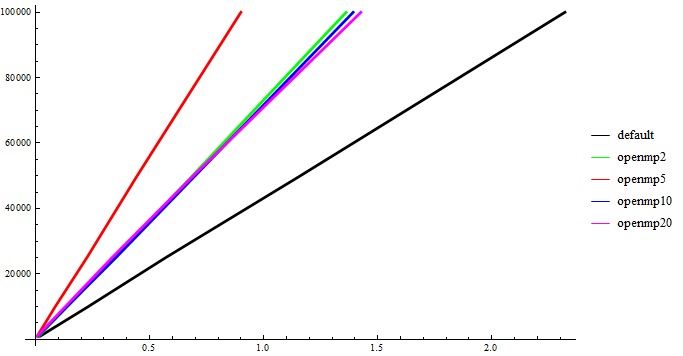
\includegraphics[width=.8\textwidth]{openmp-1}\\[1em]
  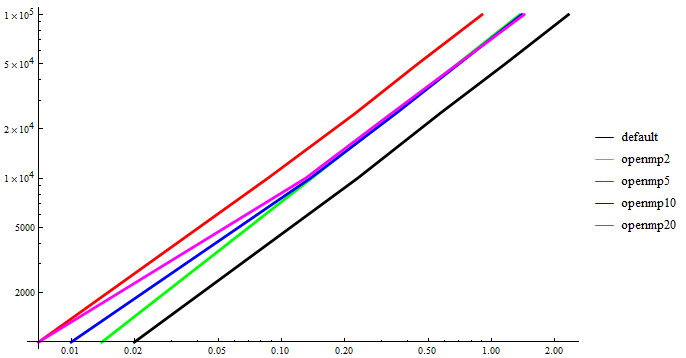
\includegraphics[width=.8\textwidth]{openmp-2}
\end{figure}

\newpage

\section{Сертификаты с Intuit}
\begin{figure}[h!]
  \centering
  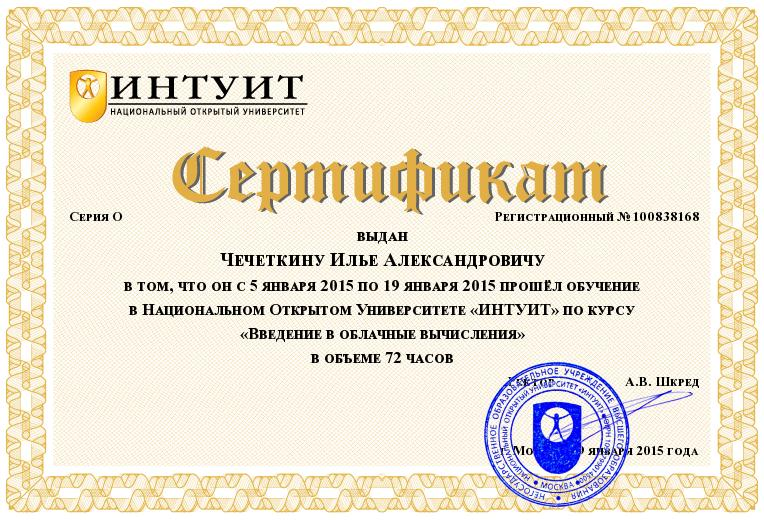
\includegraphics[width=.85\textwidth]{cloud}\\[2em]
  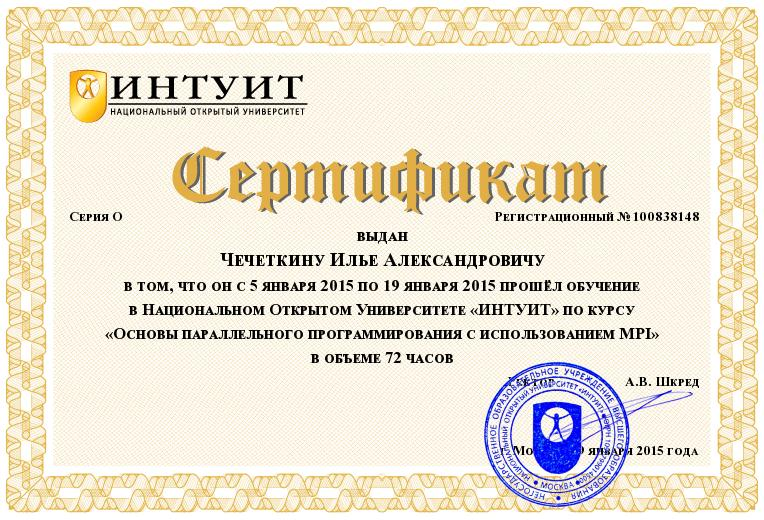
\includegraphics[width=.85\textwidth]{mpi}
\end{figure}

\newpage

\renewcommand{\bibname}{Список используемой литературы}
\addcontentsline{toc}{section}{Список используемой литературы}
\begin{thebibliography}{10}
	\bibitem{methods} Высокопроизводительные вычисления на кластерах:
	  Учебное пособие~/ Под~ред. А.~В.~Старченко.~---
	  Томск: Изд-во Том. ун-та, 2008.~--- 198~с. 
	\bibitem{Antonov} Антонов, А.~С. Параллельное программирование с использованием
	  технологии OpenMP: Учебное пособие.~/ А.~С.~Антонов, НИВЦ МГУ.~---
	  Москва: Изд-во МГУ, 2009.~--- 77~с.
	\bibitem{book1} Заусаев, А.~Ф. Применение разностных методов для решения
    обыкновенных дифференциальных уравнений: лабораторный практикум~/
    А.~Ф.~Заусаев, В.~Е.~Зотеев.~---
    Самара, Самар. гос. техн. ун-т, 2010.~--- 34~с.
\end{thebibliography}

\newpage

\end{document}
